\documentclass[conference]{IEEEtran}
\usepackage[utf8]{inputenc}
\usepackage[T1]{fontenc}
\usepackage{float,amsmath,booktabs,array,graphicx,tikz,microtype,cite}
\usetikzlibrary{arrows.meta,positioning,calc}
\renewcommand{\tablename}{Tabla}\renewcommand{\figurename}{Fig.}
\renewcommand{\refname}{Referencias}
\def\tablename{TABLA}
\newcommand{\cod}[1]{\texttt{\small #1}}
\hyphenation{multi-ciclo ins-truc-ción ins-truc-cio-nes}
\begin{document}
\title{Microarquitectura RV32I multiciclo en Verilog:\\ diseño, decodificación por formato y verificación}
\author{\IEEEauthorblockN{Isaac David Angulo Hidalgo, Adrián Espinosa Campos, Alejandro Pereira Gutiérrez, David Alejandro Rojas Castro}
\IEEEauthorblockA{Escuela de Ingeniería Mecatrónica, Tecnológico de Costa Rica\\
MT-7003 Microprocesadores y Microcontroladores, Grupo N°\,3, II Semestre 2026}}
\maketitle

\begin{abstract}
Este informe describe el diseño y la verificación de un procesador RISC-V RV32I multiciclo escrito en Verilog y simulado en Vivado. El procesador ejecuta diez instrucciones (\cod{addi, lw, slli, andi, sw, sb, lui, bne, bge, jal}), con lo que cubre los cinco formatos de instrucción I, S, B, U y J. Explicamos la ruta de datos de 20 módulos, la unidad de control (una máquina de Moore de 13 estados) y cómo se decodifica cada formato, relacionando cada módulo con la instrucción que lo justifica. Para verificarlo usamos un programa en C compilado a ensamblador: se ejecutan 42 instrucciones en 174 ciclos (CPI de 4,1) y la memoria queda con los valores que predice el código fuente.
\end{abstract}
\begin{IEEEkeywords}
RISC-V, RV32I, multiciclo, máquina de estados, Verilog, Vivado.
\end{IEEEkeywords}

\section{Introducción}
El objetivo del proyecto es construir un microprocesador que ejecute un programa real en C, compilado para RV32I \cite{spec}, y demostrar que funciona mediante simulación. No implementamos el conjunto completo de instrucciones: analizamos el programa de prueba, extrajimos las diez instrucciones que realmente usa y diseñamos el hardware justo para ellas, sin dejar de respetar el formato de cada una.

Elegimos una microarquitectura multiciclo \cite{pat}. En lugar de resolver la instrucción completa en un solo pulso de reloj, la dividimos en varios pasos, de un ciclo cada uno, y así una misma memoria, una misma ALU y un puñado de registros intermedios se reutilizan en cada paso. El módulo superior, \cod{top\_rv32i}, tiene como únicas entradas \cod{clk} y \cod{rst}, como pide el enunciado \cite{enun}, y una salida \cod{halted} que indica que el programa terminó.

El resto del documento sigue el orden en que trabajamos. La sección~II cuenta cómo llegamos al diseño final; la III describe el programa de prueba; la IV y la V presentan la ruta de datos y la unidad de control; la VI explica cómo se decodifica cada formato; la VII justifica los módulos; y la VIII muestra la verificación y los resultados. El código, los testbenches, los diagramas y la bitácora están en el repositorio del grupo \cite{repo}.

\section{Proceso de diseño}
Empezamos con una arquitectura monociclo (Avance 1). Al presentarla, el profesor nos hizo ver que el PC, la memoria, el banco de registros y la RAM dependían todos del flanco de subida, así que la instrucción y sus acciones quedaban desfasadas dentro del mismo pulso. De ahí salió la decisión de pasar a multiciclo, y en la misma reunión adoptamos GitHub para el control de versiones y la bitácora (entradas 3 y 4).

Después de rediseñar el diagrama, redactamos una especificación detallada en el \cod{README.md}: una sección por módulo con su tabla de puertos y su descripción operativa, la tabla de estados de la FSM y la tabla maestra de señales de control. Esa especificación fue la referencia para escribir el Verilog (entradas 5 a 7).

La codificación final fue incremental (entrada 8). Para cada módulo escribimos el Verilog, un testbench con su objetivo, estímulos y resultados esperados, y lo simulamos en Vivado antes de pasar al siguiente.

\section{Programa de prueba}
El programa (Fig.~\ref{fig:c}) lo compilamos con GCC para RV32I y lo recortamos a las instrucciones soportadas. Declara un puntero con el valor \cod{0xC7DF}, un carácter, un entero y un lazo de dos iteraciones: en la primera se cambia el carácter a \texttt{'b'} y en la segunda se desplaza \cod{b} un bit a la izquierda y se enmascara. Cada construcción termina ejercitando uno o más formatos.

\begin{figure}[H]
\centering\footnotesize
\begin{tabular}{@{}l@{\hspace{1.2em}}l@{}}
\texttt{int *r = 0xC7DF;} & \cod{lui, addi, sw} (U, I, S)\\
\texttt{char a = 'c';} & \cod{addi, sb} (I, S)\\
\texttt{int b = 33;} & \cod{addi, sw}\\
\texttt{for (i=0; i<2; i++)} & \cod{jal, lw, addi, sw, bge} (J, I, S, B)\\
\texttt{if (i==0) a = 'b';} & \cod{lw, bne, addi, sb, jal}\\
\texttt{b = b<<1; b = b\&0xF;} & \cod{lw, slli, sw, lw, andi, sw}
\end{tabular}
\caption{Programa en C y las instrucciones RV32I que genera.}\label{fig:c}
\end{figure}

El programa final ocupa 31 palabras (\cod{0x00}--\cod{0x78}) y se carga con \cod{\$readmemh}; el listado completo está en el Anexo~B. La palabra que sigue no está inicializada (valor \cod{x}): su \cod{opcode} no coincide con ninguna instrucción soportada y la FSM pasa a \cod{HALT}, que usamos como marca de fin.

Las variables viven en la pila. Como \cod{sp} arranca en cero, la primera instrucción (\cod{addi sp,sp,-32}) lo deja en \cod{0xFFFFFFE0}. Nuestra memoria es de 256 palabras y solo usa los bits \cod{Address[9:2]}, de modo que esa dirección cae en la palabra 248 (byte \cod{0x3E0}). El programa queda en la parte baja de la RAM, la pila en la parte alta, y no hace falta inicializar \cod{sp}.

\section{Arquitectura general}
La Fig.~\ref{fig:dp} (Anexo A) muestra el diagrama final y la Tabla~\ref{tab:mod} lista los módulos. Para entenderla conviene seguir un dato a lo largo del circuito. El \cod{PC} da la dirección a la memoria, que entrega una palabra de instrucción al registro \cod{Instrucciones}. De ahí salen los campos \cod{rs1}, \cod{rs2} y \cod{rd} hacia el banco de registros, el bloque \cod{imm\_extend} arma el inmediato, y el \cod{opcode} va a la FSM. Los operandos pasan por los registros \cod{A} y \cod{B} hasta la ALU, cuyo resultado se guarda en \cod{ALUOut}. Finalmente el multiplexor \cod{ResultSrc} decide si lo que se escribe (en el banco de registros o en el \cod{PC}) es \cod{ALUOut}, el dato leído de memoria o la salida directa de la ALU.

\begin{table}[t]
\caption{Módulos de la ruta de datos}\label{tab:mod}
\centering\footnotesize
\setlength{\tabcolsep}{3pt}\begin{tabular}{@{}p{2.9cm}p{5.4cm}@{}}\toprule
Módulo & Función\\\midrule
\cod{pc} & Contador de programa de 32 bits con habilitación \cod{PCWrite}.\\
\cod{memory} & RAM unificada de 256 palabras; lectura asíncrona y escritura síncrona por byte (\cod{ByteWrite}).\\
\cod{registers} & 32 registros de 32 bits, dos lecturas asíncronas y una escritura (\cod{RegWrite}); \cod{x0} siempre vale 0.\\
\cod{reg\_instructions} & Retiene la instrucción durante todo su ciclo de vida (\cod{IRWrite}).\\
\cod{reg\_old\_pc} & Guarda el \cod{PC} en cada flanco; en \cod{DECODE} contiene la dirección de la instrucción.\\
\cod{reg\_a, reg\_b} & Operandos \cod{rs1} y \cod{rs2} leídos en \cod{DECODE}; \cod{B} también es el dato que se escribe en memoria.\\
\cod{reg\_alu\_out} & Resultado de la ALU para el ciclo siguiente.\\
\cod{reg\_datos} & Palabra leída por \cod{lw}.\\
\cod{imm\_extend} & Reordena y extiende el inmediato según \cod{ImmSrc}.\\
\cod{alu} & ADD, SUB, AND, SLL y PASS-B; banderas \cod{Zero} y \cod{GE}.\\
\cod{mux\_*} (4) & \cod{AdrSrc}, \cod{ALUSrcA}, \cod{ALUSrcB}, \cod{ResultSrc}.\\
\cod{control\_fsm} & Máquina de Moore de 13 estados.\\
Decodificadores (\cod{alu\_}, \cod{imm\_}, \cod{byte\_}) y \cod{pc\_write\_logic} & Lógica combinacional auxiliar de control.\\\bottomrule
\end{tabular}
\end{table}

Los selectores de los multiplexores son:
\begin{itemize}
\item \cod{ALUSrcA}: 00 \cod{PC}, 01 \cod{OldPC}, 10 \cod{A}.
\item \cod{ALUSrcB}: 00 \cod{B}, 01 \cod{ImmExt}, 10 constante 4.
\item \cod{ResultSrc}: 00 \cod{ALUOut}, 01 \cod{Datos}, 10 salida directa de la ALU.
\item \cod{AdrSrc}: 0 \cod{PC}, 1 \cod{ALUOut}.
\end{itemize}

La ALU realiza las operaciones de la Tabla~\ref{tab:alu} y entrega dos banderas: \cod{Zero} (resultado nulo) y \cod{GE} (\cod{SrcA}$\ge$\cod{SrcB} interpretados con signo). Ambas van a \cod{pc\_write\_logic}.

\begin{table}[t]
\caption{Operaciones de la ALU y su decodificación}\label{tab:alu}
\centering\footnotesize
\setlength{\tabcolsep}{3pt}\begin{tabular}{@{}ccp{2.6cm}cl@{}}\toprule
\cod{ALUOp} & \cod{f3} & Instrucción & \cod{ALUCtl} & Operación\\\midrule
00 & -- & direcciones, PC+4 & 000 & ADD\\
01 & -- & \cod{bne, bge} & 001 & SUB\\
10 & 000 & \cod{addi} & 000 & ADD\\
10 & 111 & \cod{andi} & 010 & AND\\
10 & 001 & \cod{slli} & 011 & SLL\\
11 & -- & \cod{lui} & 100 & PASS-B\\\bottomrule
\end{tabular}
\end{table}

Los registros \cod{A}, \cod{B}, \cod{ALUOut} y \cod{Datos} se recargan en cada flanco de reloj y no tienen habilitación. Lo hicimos así a propósito: la FSM siempre consume cada valor en el ciclo inmediatamente siguiente a su captura, así que una habilitación solo añadiría señales de control sin cambiar el resultado. Solo \cod{PC} e \cod{Instrucciones} la necesitan, porque deben conservar su valor durante varios ciclos.

\section{Unidad de control}
\subsection{La máquina de estados}
La unidad de control (\cod{control\_fsm}) es una máquina de Moore: las salidas dependen únicamente del estado actual. Esto da selectores estables durante todo el ciclo y simplifica el análisis de tiempos. La FSM mira solo el \cod{opcode} para decidir qué estado sigue después de \cod{DECODE}; el detalle fino (\cod{funct3}, formato del inmediato, máscara de bytes) lo resuelven tres decodificadores combinacionales aparte. Gracias a esa separación bastan 13 estados para las diez instrucciones (Fig.~\ref{fig:fsm}). Cualquier \cod{opcode} no soportado, incluida una palabra sin inicializar, lleva a \cod{HALT}, estado del que solo se sale con un reset.

\begin{figure*}[t]
\centering
\resizebox{0.97\textwidth}{!}{%
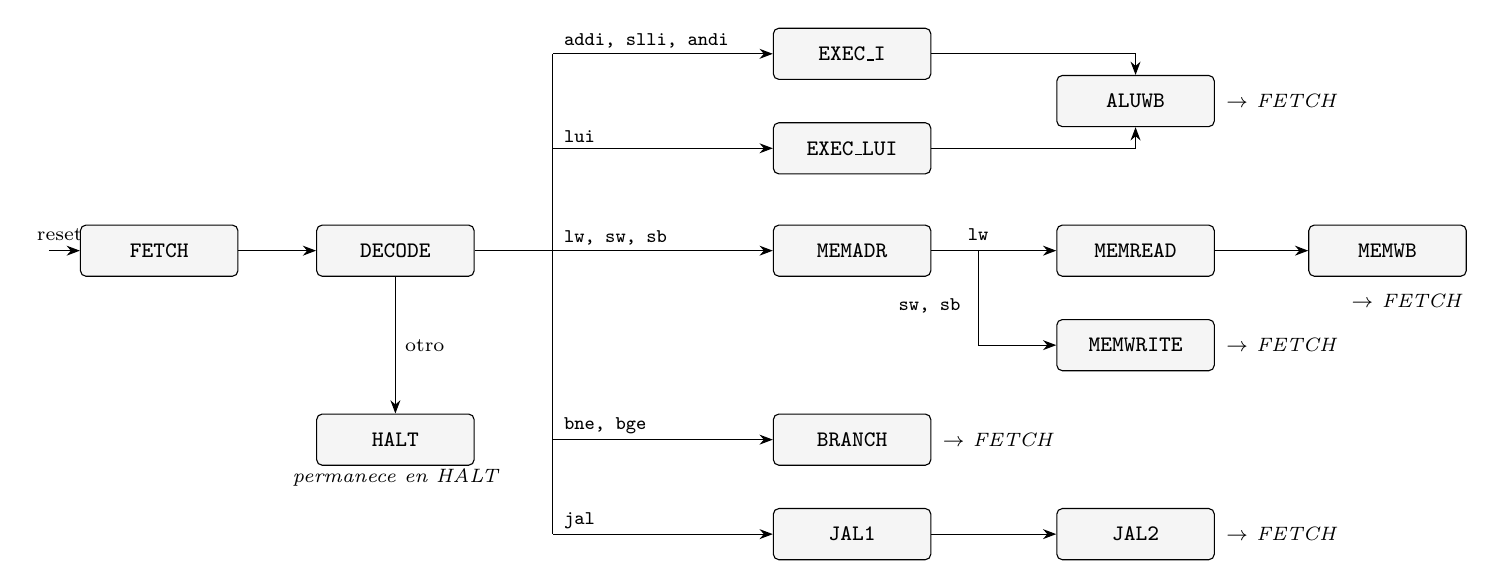
\begin{tikzpicture}[>=Stealth,x=1cm,y=1cm,
 st/.style={draw,rounded corners=2pt,minimum width=20mm,minimum height=6.5mm,font=\footnotesize\ttfamily,inner sep=2pt,fill=gray!8},
 lb/.style={font=\scriptsize\ttfamily,inner sep=1pt,anchor=south west},
 rt/.style={font=\scriptsize\itshape,inner sep=1pt,anchor=west}]
\def\tx{5.0}
\node[st] (F) at (0,0) {FETCH};
\node[st] (D) at (3.0,0) {DECODE};
\node[st] (EI) at (8.8,2.5) {EXEC\_I};
\node[st] (EL) at (8.8,1.3) {EXEC\_LUI};
\node[st] (AW) at (12.4,1.9) {ALUWB};
\node[st] (MA) at (8.8,0) {MEMADR};
\node[st] (MR) at (12.4,0) {MEMREAD};
\node[st] (MW) at (15.6,0) {MEMWB};
\node[st] (MS) at (12.4,-1.2) {MEMWRITE};
\node[st] (BR) at (8.8,-2.4) {BRANCH};
\node[st] (J1) at (8.8,-3.6) {JAL1};
\node[st] (J2) at (12.4,-3.6) {JAL2};
\node[st] (H) at (3.0,-2.4) {HALT};
% flechas principales
\draw[->] (-1.4,0)--(F) node[pos=0.35,above,font=\scriptsize]{reset};
\draw[->] (F)--(D);
\draw (D.east)--(\tx,0);
\draw (\tx,2.5)--(\tx,-3.6);
\foreach \y/\n/\t in {2.5/EI/{addi, slli, andi},1.3/EL/{lui},0/MA/{lw, sw, sb},-2.4/BR/{bne, bge},-3.6/J1/{jal}}{
  \draw[->] (\tx,\y)--(\n.west);
  \node[lb] at (\tx+0.1,\y+0.03) {\t};
}
\draw[->] (D.south)--(H.north) node[font=\scriptsize,midway,right]{otro};
\node[rt,anchor=north] at (H.south) {permanece en HALT};
\draw[->] (EI.east)-|(AW.north);
\draw[->] (EL.east)-|(AW.south);
\draw[->] (MA.east)--(MR.west) node[font=\scriptsize\ttfamily,midway,above,xshift=-2mm]{lw};
\draw[->] (MR.east)--(MW.west);
\draw[->] (10.4,0)--(10.4,-1.2)--(MS.west);
\node[font=\scriptsize\ttfamily,anchor=east] at (10.3,-0.7) {sw, sb};
\draw[->] (J1.east)--(J2.west);
\node[rt] at ($(AW.east)+(1mm,0)$) {$\to$ FETCH};
\node[rt] at ($(MW.south)+(-5mm,-3mm)$) {$\to$ FETCH};
\node[rt] at ($(MS.east)+(1mm,0)$) {$\to$ FETCH};
\node[rt] at ($(BR.east)+(1mm,0)$) {$\to$ FETCH};
\node[rt] at ($(J2.east)+(1mm,0)$) {$\to$ FETCH};
\end{tikzpicture}}
\caption{Diagrama de estados de la FSM. Los estados que terminan una instrucción regresan a \cod{FETCH}.}\label{fig:fsm}
\end{figure*}

\subsection{Qué pasa en cada ciclo}
Los dos primeros ciclos son iguales para todas las instrucciones. En \cod{FETCH} se lee \cod{Mem[PC]} hacia \cod{Instrucciones}, y al mismo tiempo la ALU calcula \cod{PC+4} y lo escribe en el \cod{PC} usando la salida directa (\cod{ResultSrc}=10), sin pasar por \cod{ALUOut}. En \cod{DECODE} se leen \cod{rs1} y \cod{rs2} hacia \cod{A} y \cod{B}; como la ALU está libre, aprovechamos para calcular \cod{OldPC+ImmExt} y dejarlo en \cod{ALUOut}. Ese valor es el destino de \cod{bne}, \cod{bge} y \cod{jal}; en las demás instrucciones simplemente se descarta. A partir de ahí cada instrucción sigue su camino (Tabla~\ref{tab:fsm}), y la duración resultante aparece en la Tabla~\ref{tab:cpi}.

Como ejemplo, la Tabla~\ref{tab:lw} sigue \cod{lw a5,-24(s0)} (\cod{0xFE842783}, en \cod{0x34}) durante sus cinco ciclos, en la primera pasada del lazo, cuando \cod{s0}=0 y \cod{i}=0.

\begin{table}[t]
\caption{Traza de \cod{lw a5,-24(s0)} en \cod{0x34}}\label{tab:lw}
\centering\footnotesize
\setlength{\tabcolsep}{3pt}\begin{tabular}{@{}clp{5.2cm}@{}}\toprule
Ciclo & Estado & Efecto al terminar el ciclo\\\midrule
1 & \cod{FETCH} & \cod{Instrucciones}$\leftarrow$\cod{0xFE842783}; \cod{PC}$\leftarrow$\cod{0x38}; \cod{OldPC}$\leftarrow$\cod{0x34}\\
2 & \cod{DECODE} & \cod{A}$\leftarrow$\cod{s0}=0; \cod{ALUOut}$\leftarrow$\cod{0x34}$-$24 (descartado)\\
3 & \cod{MEMADR} & \cod{ALUOut}$\leftarrow$\cod{A}+(-24)=\cod{0xFFFFFFE8}\\
4 & \cod{MEMREAD} & Dirección=\cod{ALUOut}; \cod{Datos}$\leftarrow$\cod{Mem[0x3E8]}=0 (valor de \cod{i})\\
5 & \cod{MEMWB} & \cod{a5}$\leftarrow$\cod{Datos}\\\bottomrule
\end{tabular}
\end{table}

\begin{table*}[t]
\caption{Señales activas por estado (las no listadas valen 0)}\label{tab:fsm}
\centering\footnotesize
\begin{tabular}{@{}lll@{}}\toprule
Estado & Señales de control & Siguiente\\\midrule
FETCH & IRWrite, PCUpdate, ALUSrcA=00, ALUSrcB=10, ALUOp=00, ResultSrc=10 & DECODE\\
DECODE & ALUSrcA=01 (OldPC), ALUSrcB=01 (ImmExt), ALUOp=00 & según \cod{opcode}\\
MEMADR & ALUSrcA=10 (A), ALUSrcB=01, ALUOp=00 & MEMREAD (\cod{lw}) / MEMWRITE (\cod{sw, sb})\\
MEMREAD & AdrSrc=1 & MEMWB\\
MEMWB & ResultSrc=01, RegWrite & FETCH\\
MEMWRITE & AdrSrc=1, MemWrite (\cod{ByteWrite} lo fija \cod{byte\_decoder}) & FETCH\\
EXEC\_I & ALUSrcA=10, ALUSrcB=01, ALUOp=10 (según \cod{funct3}) & ALUWB\\
EXEC\_LUI & ALUSrcB=01, ALUOp=11 (PASS-B) & ALUWB\\
ALUWB & ResultSrc=00, RegWrite & FETCH\\
BRANCH & ALUSrcA=10, ALUSrcB=00, ALUOp=01, Branch, ResultSrc=00 & FETCH\\
JAL1 & PCUpdate, ResultSrc=00 & JAL2\\
JAL2 & ALUSrcA=01, ALUSrcB=10, ALUOp=00, ResultSrc=10, RegWrite & FETCH\\
HALT & halted=1, sin escrituras & HALT\\\bottomrule
\end{tabular}
\end{table*}

\begin{table}[t]
\caption{Ciclos por instrucción y frecuencia en el programa}\label{tab:cpi}
\centering\footnotesize
\begin{tabular}{@{}lccc@{}}\toprule
Instrucción & Ciclos & Veces & Ciclos totales\\\midrule
\cod{addi} & 4 & 12 & 48\\
\cod{lw} & 5 & 9 & 45\\
\cod{sw} & 4 & 9 & 36\\
\cod{sb} & 4 & 2 & 8\\
\cod{lui} & 4 & 1 & 4\\
\cod{slli}, \cod{andi} & 4 & 1+1 & 8\\
\cod{jal} & 4 & 2 & 8\\
\cod{bne} & 3 & 2 & 6\\
\cod{bge} & 3 & 3 & 9\\\midrule
Total & & 42 & 172\\\bottomrule
\end{tabular}
\end{table}

\section{Decodificación por formato}
Un mismo cableado debe interpretar cinco formatos distintos, y la diferencia principal está en cómo se reparten los bits del inmediato (Tabla~\ref{tab:fmt}). El decodificador \cod{imm\_decoder} deduce el formato solo del \cod{opcode} y entrega \cod{ImmSrc} a \cod{imm\_extend}, que reordena \cod{Instr[31:7]} y extiende el signo desde \cod{Instr[31]}.

\begin{table}[t]
\caption{Formatos soportados y construcción del inmediato}\label{tab:fmt}
\centering\footnotesize
\setlength{\tabcolsep}{2.5pt}\begin{tabular}{@{}clp{4.3cm}@{}}\toprule
\cod{ImmSrc} & Formato & Inmediato\\\midrule
000 & I & \cod{Instr[31:20]}\\
001 & S & \cod{Instr[31:25]}, \cod{Instr[11:7]}\\
010 & B & \cod{Instr[31]}, \cod{[7]}, \cod{[30:25]}, \cod{[11:8]}, bit 0 = 0\\
011 & J & \cod{Instr[31]}, \cod{[19:12]}, \cod{[20]}, \cod{[30:21]}, bit 0 = 0\\
100 & U & \cod{Instr[31:12]} seguido de 12 ceros\\\bottomrule
\end{tabular}
\end{table}

\subsection{Tipo I: \cod{addi}, \cod{lw}, \cod{slli}, \cod{andi}}
Tres de estas instrucciones son aritméticas con inmediato y siguen el camino \cod{EXEC\_I}: la ALU opera \cod{A} con \cod{ImmExt} y \cod{alu\_decoder} (\cod{ALUOp}=10) escoge la operación según \cod{funct3}: suma (000) para \cod{addi}, AND (111) para \cod{andi} y desplazamiento lógico a la izquierda (001) para \cod{slli}. \cod{lw} comparte el formato, pero usa la ALU para calcular la dirección \cod{A+ImmExt} en \cod{MEMADR}; el dato leído se captura en \cod{Datos} y se escribe en \cod{rd} con \cod{ResultSrc}=01.

\subsection{Tipo S: \cod{sw}, \cod{sb}}
En el formato S el inmediato se parte en dos pedazos porque \cod{rs2} ocupa la posición donde otros formatos ponen bits bajos. \cod{MEMADR} calcula \cod{A+ImmExt} y \cod{MEMWRITE} escribe \cod{B}. Lo delicado es la escritura parcial: \cod{byte\_decoder} produce \cod{ByteWrite} de 4 bits, con 1111 para \cod{sw} y para \cod{sb} un solo bit activo según \cod{Address[1:0]} (0001, 0010, 0100 u 1000). En el programa, \cod{sb a5,-29(s0)} escribe en la dirección \cod{0x3E3}, así que activa el byte 3 (1000) y el resto de la palabra queda intacto.

\subsection{Tipo B: \cod{bne}, \cod{bge}}
El destino del salto ya está en \cod{ALUOut} desde \cod{DECODE}, por lo que \cod{BRANCH} solo tiene que decidir si se toma. La ALU resta \cod{A}$-$\cod{B} y genera \cod{Zero} y \cod{GE}; \cod{pc\_write\_logic} las combina con \cod{funct3}:
\begin{equation}
\begin{split}\mathit{PCWrite}=\mathit{PCUpdate}\lor \mathit{Branch}\land\big[&(f3{=}001\land\overline{Zero})\\&\lor(f3{=}101\land GE)\big]\end{split}
\end{equation}
Si la condición se cumple, el \cod{PC} carga \cod{ALUOut}; si no, conserva el \cod{PC+4} que escribió \cod{FETCH}. Por eso estas instrucciones tardan solo 3 ciclos.

Tomemos \cod{bge a5,a4,-64} (\cod{0xFCE7D0E3}, en \cod{0x74}), la que cierra el lazo. Antes se ejecutó \cod{addi a5,x0,1}, así que \cod{a5}=1. En \cod{DECODE}, \cod{ALUOut}=\cod{0x74}$-$64=\cod{0x34}. Si $a5\ge a4$ (con signo), \cod{GE}=1 y el \cod{PC} salta a \cod{0x34}, el inicio del lazo; si no, el programa continúa en \cod{0x78}. Con \cod{i}=0 y \cod{i}=1 salta, con \cod{i}=2 sale. Necesitamos la bandera \cod{GE} porque la comparación con signo no se puede deducir de \cod{Zero}.

\subsection{Tipo U: \cod{lui}}
\cod{lui} coloca un inmediato de 20 bits en la parte alta del registro. En vez de añadir un camino especial, dejamos pasar el inmediato por la ALU con una operación PASS-B (\cod{ALUOp}=11): en \cod{EXEC\_LUI} el resultado es \cod{ImmExt}, y \cod{ALUWB} lo escribe en \cod{rd}. El programa usa \cod{lui a5,0xC} seguido de \cod{addi a5,a5,2015} para armar \cod{0xC7DF}, que es lo que se guarda en la variable \cod{r}.

\subsection{Tipo J: \cod{jal}}
El inmediato de 21 bits se reconstruye con el bit 0 en cero. \cod{jal} tiene que hacer dos cosas, cambiar el \cod{PC} y guardar la dirección de retorno en \cod{rd}, pero solo disponemos de un multiplexor \cod{Result} que alimenta ambos destinos. Por eso lo dividimos en dos estados: \cod{JAL1} carga el \cod{PC} con el destino ya calculado en \cod{ALUOut} (\cod{PCUpdate}=1, \cod{ResultSrc}=00) y \cod{JAL2} calcula \cod{OldPC+4} y lo escribe en \cod{rd} (\cod{ALUSrcA}=01, \cod{ALUSrcB}=10, \cod{ResultSrc}=10). En ambos estados se usa el mismo multiplexor; lo único que cambia es el destino. El programa usa \cod{jal} con \cod{rd}=\cod{x0}, es decir, como un salto simple. Por ejemplo, \cod{0x03C0006F} en \cod{0x30} salta al destino \cod{0x6C}.

\section{Justificación de módulos}
Cada módulo del diseño está ahí por una instrucción concreta. Los que más conviene recordar son:
\begin{itemize}
\item \cod{OldPC}: cuando termina \cod{FETCH}, el \cod{PC} ya vale \cod{PC+4}, pero \cod{bne}, \cod{bge} y \cod{jal} necesitan la dirección original de la instrucción para sumarle el inmediato.
\item Constante 4 en \cod{ALUSrcB}: se usa en \cod{FETCH} para \cod{PC+4} y en \cod{JAL2} para la dirección de retorno.
\item \cod{ResultSrc}=10: permite escribir \cod{PC+4} en el \cod{PC} en el mismo ciclo en que se calcula, sin esperar a \cod{ALUOut}.
\item Cálculo anticipado en \cod{DECODE}: obtiene el destino de los saltos sin un sumador dedicado y sin un ciclo adicional.
\item Bandera \cod{GE}: es lo que necesita \cod{bge}, que compara con signo.
\item PASS-B: da \cod{lui} sin hardware nuevo.
\item \cod{ByteWrite}: \cod{sb} debe cambiar un solo byte sin alterar los otros tres de la palabra.
\item \cod{Datos}: mantiene el valor leído por \cod{lw} entre \cod{MEMREAD} y \cod{MEMWB}.
\item \cod{halted}: avisa que el programa terminó y dispara el volcado de memoria del testbench.
\end{itemize}

\section{Verificación y resultados}
\subsection{Pruebas por módulo}
Cada módulo tiene su testbench en \cod{sim/}, y en el encabezado de cada uno documentamos el objetivo, los estímulos en el tiempo y los resultados esperados, como pide el enunciado. La Tabla~\ref{tab:tb} resume qué se comprueba en los más importantes. Los demás (multiplexores y registros) verifican que cada selector entregue la entrada correcta y que cada registro capture, retenga y se reinicie como corresponde.

\begin{table}[t]
\caption{Pruebas de los módulos principales}\label{tab:tb}
\centering\footnotesize
\setlength{\tabcolsep}{3pt}\begin{tabular}{@{}p{3.1cm}p{5.2cm}@{}}\toprule
Testbench & Qué verifica\\\midrule
\cod{alu\_tb} & ADD, SUB, AND, SLL y PASS-B; \cod{Zero}; \cod{GE} con operandos negativos (por ejemplo $-5\ge-10$).\\
\cod{imm\_extend\_tb} & Los cinco formatos con inmediatos positivos y negativos, p. ej. \cod{0xFFFFFFFC} para $-4$ y \cod{0xC7DF0000} para \cod{lui}.\\
\cod{memory\_tb} & \cod{sw} de \cod{0xDEADBEEF}, luego \cod{sb} en el byte 0 (\cod{0xDEADBEAA}) y en el byte 2 (\cod{0xDE55BEAA}).\\
\cod{byte\_decoder\_tb} & \cod{ByteWrite}=0000 sin escritura, 1111 para \cod{sw} y los cuatro casos de \cod{sb}.\\
\cod{registers\_tb} & Lectura dual, escritura sin \cod{RegWrite} y que \cod{x0} no se modifique.\\
\cod{pc\_write\_logic\_tb} & \cod{bne} y \cod{bge} tomados y no tomados, \cod{PCUpdate} incondicional y \cod{funct3} no válido.\\
\cod{control\_fsm\_tb} & Recorrido de estados y señales de cada tipo de instrucción, y entrada y salida de \cod{HALT}.\\\bottomrule
\end{tabular}
\end{table}

\subsection{Procesador completo}
El testbench \cod{top\_rv32i\_tb} libera el reset a los 20\,ns con un reloj de 10\,ns, vigila \cod{halted} y, cuando se activa, vuelca la memoria a un archivo.

\subsection{Resultados}
El programa de 31 palabras ejecuta 42 instrucciones y llega a \cod{HALT} a los 1765\,ns, es decir 174 ciclos: los 172 de la Tabla~\ref{tab:cpi} más \cod{FETCH} y \cod{DECODE} de la palabra sin inicializar. El CPI medio es $172/42\approx4{,}10$, y las tres instrucciones más frecuentes (\cod{addi}, \cod{sw} y \cod{lw}) suman el 75\,\% de los ciclos.

El estado final de la memoria coincide con lo que predice el código C (Tabla~\ref{tab:mem}): \cod{r}=\cod{0xC7DF}; \cod{i}=2, porque el lazo termina cuando \cod{i} deja de ser menor que 2; y \cod{b}=2, ya que $33\ll1=66$ y $66\,\&\,15=2$. Además \cod{sp}=\cod{0xFFFFFFE0}, \cod{s0}=0 y \cod{a5}=0 por el \cod{li a5,0} final, y las palabras del programa (\cod{0x0}--\cod{0x78}) permanecen intactas.

\begin{table}[t]
\caption{Variables en memoria al finalizar la simulación}\label{tab:mem}
\centering\footnotesize
\begin{tabular}{@{}lll@{}}\toprule
Dirección & Valor & Variable\\\midrule
\cod{0x3E0} & \cod{0x62xxxxxx} & \cod{a} = \texttt{'b'} (byte 3)\\
\cod{0x3E4} & \cod{0x0000C7DF} & \cod{r}\\
\cod{0x3E8} & \cod{0x00000002} & \cod{i}\\
\cod{0x3EC} & \cod{0x00000002} & \cod{b}\\
\cod{0x3F8} & \cod{0x00000000} & \cod{s0} guardado\\
\cod{0x3FC} & \cod{0x00000000} & \cod{ra} guardado\\\bottomrule
\end{tabular}
\end{table}

\subsection{Análisis}
El valor de \cod{0x3E0} es la prueba más clara de que la escritura por bytes funciona. Solo el byte 3 es válido (\cod{0x62}, la letra \texttt{'b'}); los otros tres siguen indefinidos porque la memoria no se inicializa en cero. Si \cod{sb} hubiera escrito la palabra completa, esos bytes tendrían valores definidos. Además el programa escribe \texttt{'c'} (\cod{0x63}) y luego \texttt{'b'} en el mismo byte, y el segundo valor es el que prevalece, como debe ser.

Los valores de \cod{i} y \cod{b} confirman que \cod{lw}, \cod{addi}, \cod{slli}, \cod{andi} y \cod{sw} se encadenan bien a través de la memoria, y que \cod{bge} y \cod{bne} saltan o no según corresponde. Si alguno fallara, el lazo no terminaría en la segunda vuelta o \cod{b} no valdría 2.

El precio de esta arquitectura es el CPI de 4,1: cada instrucción tarda entre 3 y 5 ciclos y el procesador nunca hace dos cosas a la vez. A cambio, el hardware es pequeño. Tiene una sola ALU, una sola memoria y un solo puerto de escritura al banco de registros, y la unidad de control cabe en 13 estados.

\section{Conclusiones}
Logramos un procesador RV32I multiciclo que ejecuta completo el programa de prueba, con los cinco formatos de instrucción (I, S, B, U y J), y que deja la memoria exactamente en el estado que predice el código en C: \cod{r}=\cod{0xC7DF}, \cod{i}=2, \cod{b}=2 y el carácter \texttt{'b'} en el byte 3 de \cod{0x3E0}. El módulo superior cumple lo que pide el enunciado: solo recibe \cod{clk} y \cod{rst}, y las 42 instrucciones se resuelven en 174 ciclos hasta que la FSM llega a \cod{HALT}.

En cuanto al diseño, tres decisiones explican la mayor parte del resultado. La primera es separar una FSM mínima, que solo mira el \cod{opcode}, de decodificadores combinacionales para \cod{funct3}, el formato del inmediato y la máscara de bytes: así bastaron 13 estados en lugar de uno por cada variante de instrucción. La segunda es reutilizar la ALU en todos los ciclos (\cod{PC+4}, destino de salto, dirección efectiva y el paso de \cod{lui}), lo que evitó sumadores adicionales y mantuvo la ruta de datos con una sola unidad aritmética. La tercera es calcular el destino de los saltos durante \cod{DECODE}, de modo que \cod{bne} y \cod{bge} necesitan solo tres ciclos y \cod{jal} se resuelve con dos estados que comparten el mismo multiplexor de resultado.

Estas decisiones tienen un costo medible: un CPI de 4,1, con instrucciones de 3 a 5 ciclos. Es el precio de usar una sola memoria, una sola ALU y un solo puerto de escritura, a cambio de un circuito pequeño y fácil de verificar módulo por módulo, que fue justamente lo que permitió llegar a la integración con confianza en cada pieza.

Además de los resultados, el proyecto nos permitió ver cómo cada decisión de la microarquitectura se refleja en una instrucción concreta: el registro \cod{OldPC} existe por los saltos, la bandera \cod{GE} por \cod{bge}, la operación PASS-B por \cod{lui} y la máscara \cod{ByteWrite} por \cod{sb}. La bitácora y el repositorio dejan constancia de ese proceso de diseño y de las decisiones del grupo.

\begin{thebibliography}{1}
\bibitem{spec} A.~Waterman and K.~Asanović, \emph{The RISC-V Instruction Set Manual, Vol.~I: Unprivileged ISA}, RISC-V International.
\bibitem{pat} D.~Patterson and A.~Waterman, \emph{The RISC-V Reader: An Open Architecture Atlas}, Strawberry Canyon, 2017.
\bibitem{enun} C.~Salazar García, \emph{Proyecto: Microprocesador RV32I}, MT-7003, Tecnológico de Costa Rica, II Sem. 2026.
\bibitem{repo} Grupo N°\,3, ``mt7003-riscv-vivado-implementation,'' repositorio \texttt{davidrojas0/mt7003-riscv-vivado-implementation}, rama \texttt{main}.
\end{thebibliography}

\clearpage
\onecolumn
\appendices
\section{Diagrama de la microarquitectura}
\begin{center}
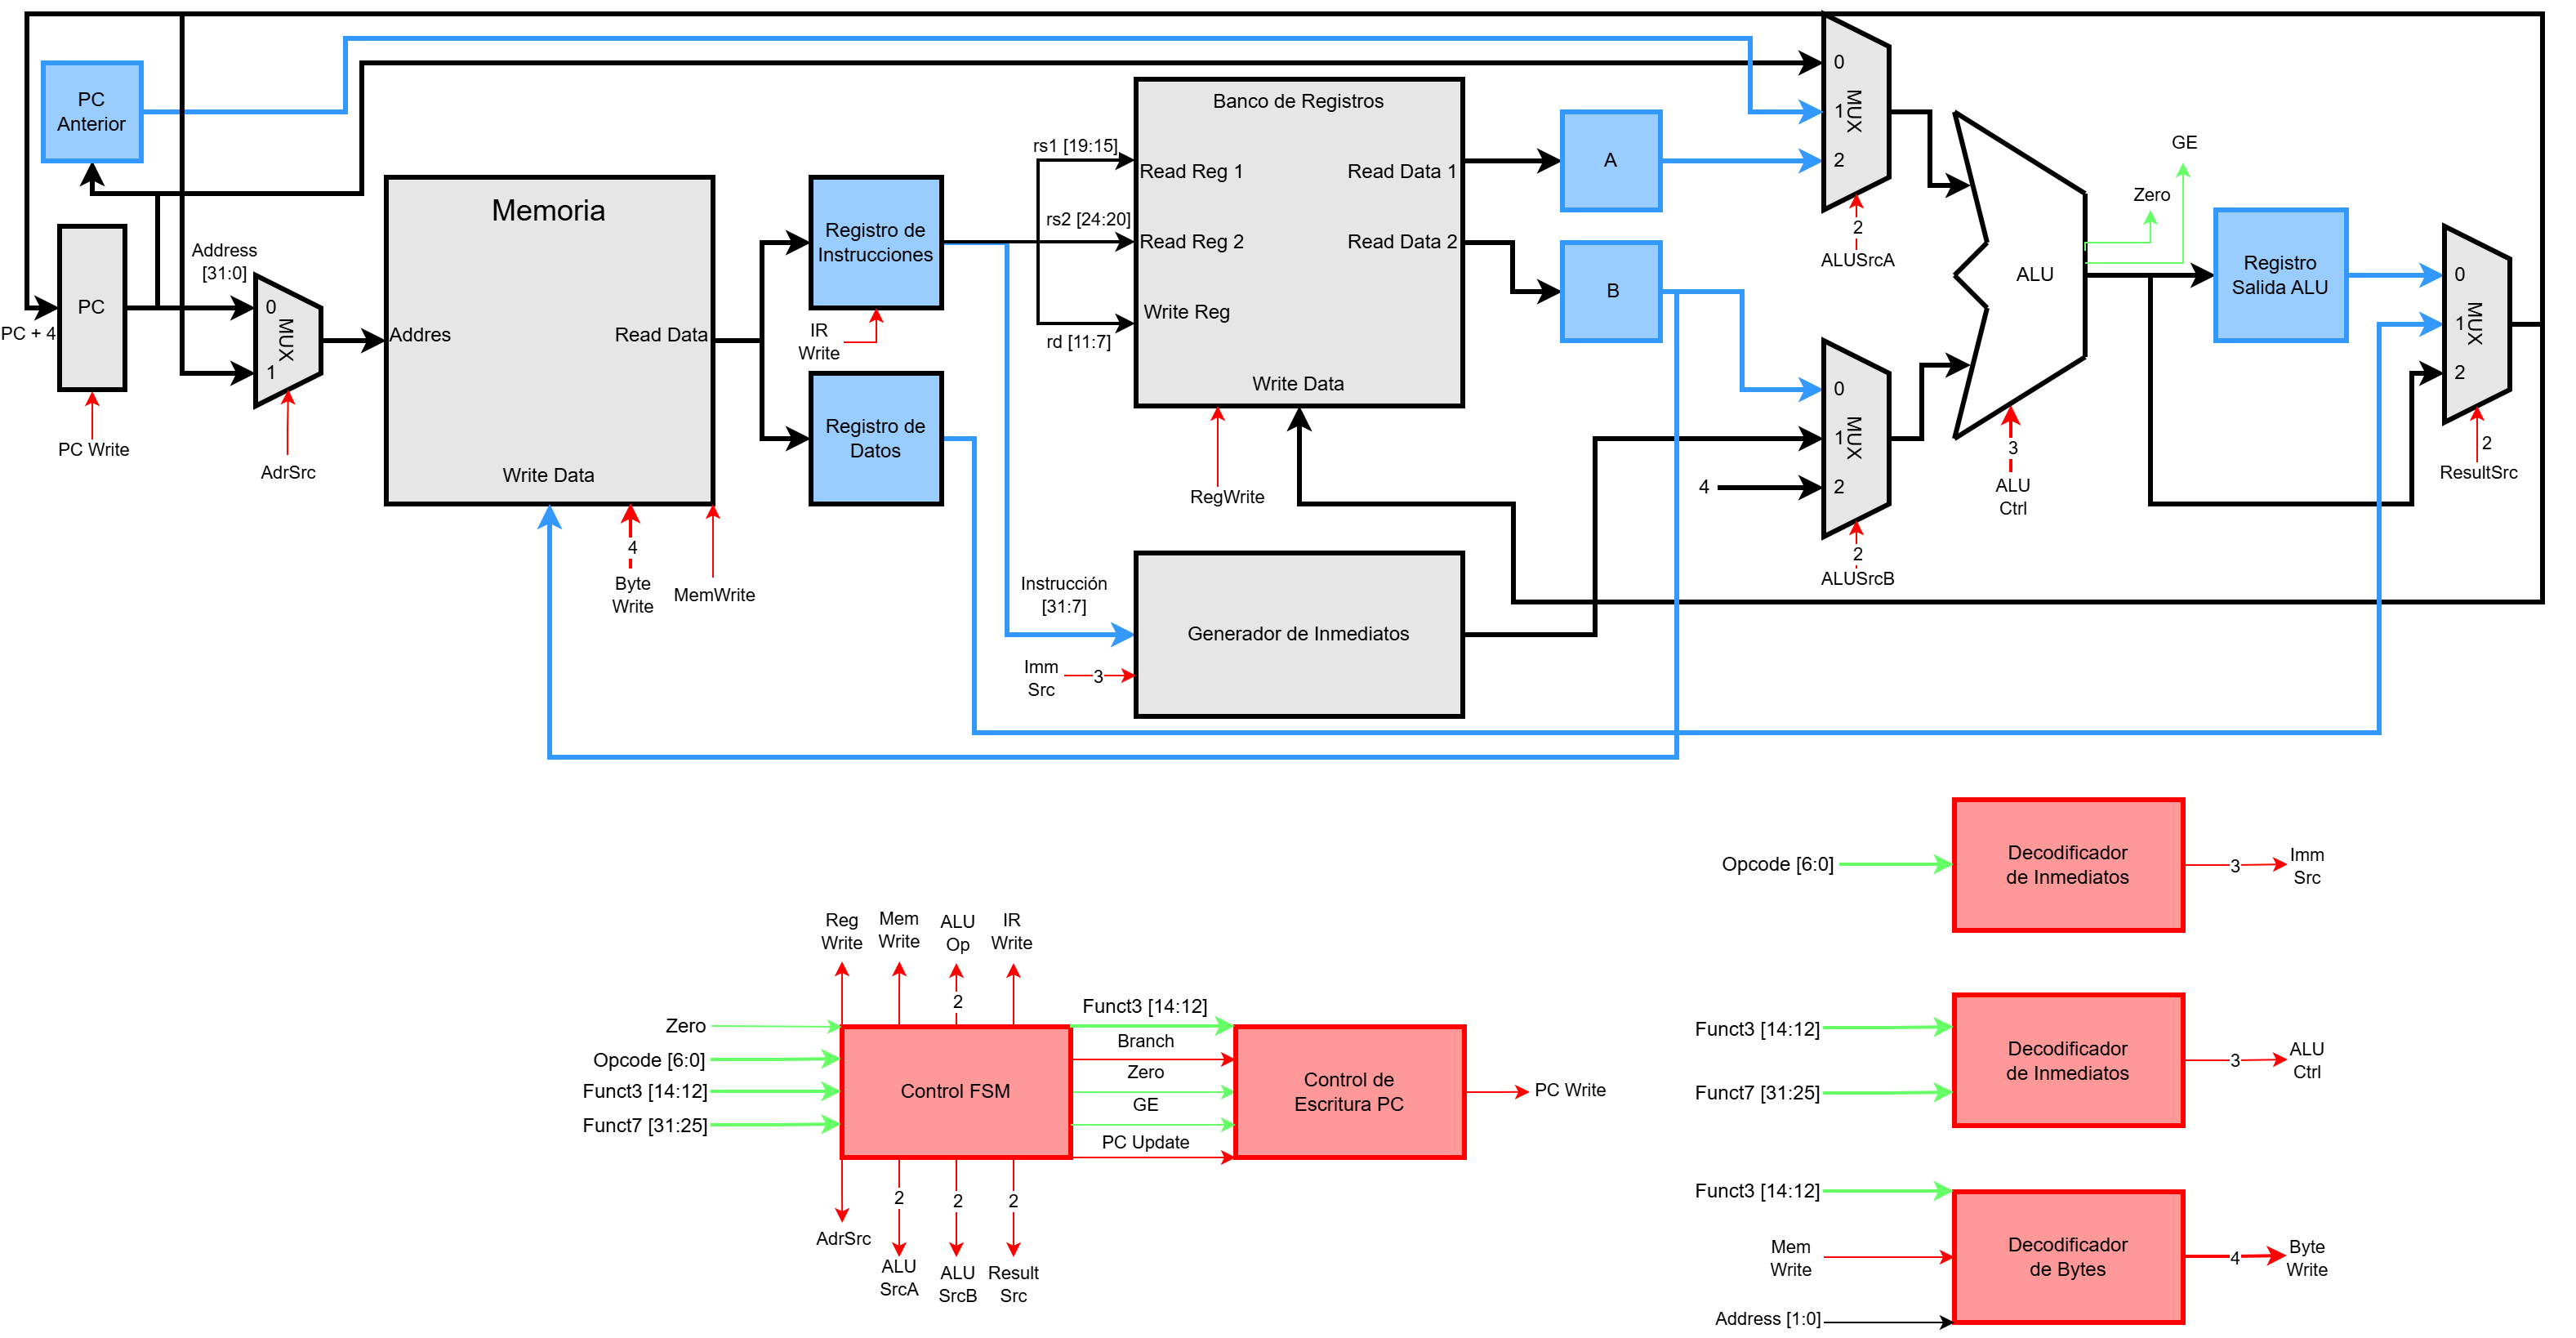
\includegraphics[width=\textwidth]{fig_final.png}\\[4pt]
\refstepcounter{figure}\footnotesize Fig.~\thefigure.\ Ruta de datos multiciclo final con unidad de control.\label{fig:dp}
\end{center}

\section{Programa de prueba y contenido inicial de la memoria}
\begin{center}
\footnotesize\setlength{\tabcolsep}{4pt}
\begin{tabular}{@{}lll@{\hspace{2em}}lll@{}}\toprule
Dir. & Palabra & Instrucción & Dir. & Palabra & Instrucción\\\midrule
\cod{0x00} & \cod{FE010113} & \cod{addi sp,sp,-32} & \cod{0x40} & \cod{FEF401A3} & \cod{sb a5,-29(s0)}\\
\cod{0x04} & \cod{00112E23} & \cod{sw ra,28(sp)} & \cod{0x44} & \cod{01C0006F} & \cod{jal x0,+0x1c}\\
\cod{0x08} & \cod{00812C23} & \cod{sw s0,24(sp)} & \cod{0x48} & \cod{FEC42783} & \cod{lw a5,-20(s0)}\\
\cod{0x0C} & \cod{02010413} & \cod{addi s0,sp,32} & \cod{0x4C} & \cod{00179793} & \cod{slli a5,a5,1}\\
\cod{0x10} & \cod{0000C7B7} & \cod{lui a5,0xc} & \cod{0x50} & \cod{FEF42623} & \cod{sw a5,-20(s0)}\\
\cod{0x14} & \cod{7DF78793} & \cod{addi a5,a5,2015} & \cod{0x54} & \cod{FEC42783} & \cod{lw a5,-20(s0)}\\
\cod{0x18} & \cod{FEF42223} & \cod{sw a5,-28(s0)} & \cod{0x58} & \cod{00F7F793} & \cod{andi a5,a5,15}\\
\cod{0x1C} & \cod{06300793} & \cod{addi a5,x0,99} & \cod{0x5C} & \cod{FEF42623} & \cod{sw a5,-20(s0)}\\
\cod{0x20} & \cod{FEF401A3} & \cod{sb a5,-29(s0)} & \cod{0x60} & \cod{FE842783} & \cod{lw a5,-24(s0)}\\
\cod{0x24} & \cod{02100793} & \cod{addi a5,x0,33} & \cod{0x64} & \cod{00178793} & \cod{addi a5,a5,1}\\
\cod{0x28} & \cod{FEF42623} & \cod{sw a5,-20(s0)} & \cod{0x68} & \cod{FEF42423} & \cod{sw a5,-24(s0)}\\
\cod{0x2C} & \cod{FE042423} & \cod{sw x0,-24(s0)} & \cod{0x6C} & \cod{FE842703} & \cod{lw a4,-24(s0)}\\
\cod{0x30} & \cod{03C0006F} & \cod{jal x0,+0x3c} & \cod{0x70} & \cod{00100793} & \cod{addi a5,x0,1}\\
\cod{0x34} & \cod{FE842783} & \cod{lw a5,-24(s0)} & \cod{0x74} & \cod{FCE7D0E3} & \cod{bge a5,a4,-64}\\
\cod{0x38} & \cod{00079863} & \cod{bne a5,x0,+0x10} & \cod{0x78} & \cod{00000793} & \cod{addi a5,x0,0}\\
\cod{0x3C} & \cod{06200793} & \cod{addi a5,x0,98} &  & & \\
\\\bottomrule
\end{tabular}

\smallskip\footnotesize La palabra \cod{0x7C} y las siguientes no se inicializan (\cod{x}); su \cod{opcode} indefinido lleva a la FSM al estado \cod{HALT}.
\end{center}
\end{document}
